\documentclass[11pt]{article}
\usepackage{fullpage}
\usepackage{graphicx}
\usepackage{subfigure}
\usepackage{comment}
\interfootnotelinepenalty=10000
\newcommand{\HRule}{\rule{\linewidth}{0.5mm}}


%numeroter les pages
\pagestyle{plain}


\begin{document}

\begin{titlepage}

\begin{center}

% Upper part of the page

 

\includegraphics[width=0.8\textwidth]{./header}\\[1cm]
\textsc{\Large Master research Internship}
\vspace{1cm}

\includegraphics[height=0.1\textheight]{./logos/cerv_2}
\includegraphics[height=0.1\textheight]{./logos/teeside}
\includegraphics[height=0.1\textheight]{./logos/fiu}
\includegraphics[height=0.1\textheight]{./logos/CHRU_Brest}


  
\vspace{1cm} 
\textsc{\Large Bibliographic report }\\[0.5cm]


% The title of your report
\HRule \\[0.4cm]
{ \Large \bfseries Virtual Reality and Schizophrenia }\\[0.4cm]
{ \bfseries Therapeutic game based on  narrative generation techniques }\\[0.2cm]
\HRule \\[1.5cm]
% The domain of your research 
\begin{flushleft}
\textbf{Domain : Human-Computer Interaction - Artificial Intelligence \\[1cm]}
\end{flushleft}


% Author and supervisor(s)
\begin{minipage}{0.4\textwidth}
\begin{flushleft} \large
\emph{Author:}\\
Cindy  \textsc{Even}
\end{flushleft}
\end{minipage}
\begin{minipage}{0.4\textwidth}
\begin{flushright} \large
\emph{Supervisors:} \\[2ex]
%
% name(s) of your supervisor(s)
Anne-Gwenn \textsc{Bosser } \\
C\'{e}dric \textsc{Buche } \\
% Name of your team
IHSEV - Lab-STICC - France\\[2ex]
Jo\~{a}o \textsc{F. Ferreira } \\
Digital Futures Institute - UK
\end{flushright}
\end{minipage}

\vfill


% INCLUDE HERE THE LOGO OF YOUR INSTITUTION
\begin{flushleft}
\includegraphics[width=0.2\textwidth]{./logos/enib}
\end{flushleft}
\end{center}
\end{titlepage}

%************************************************************%

\begin{abstract}
Patients suffering from schizophrenia and related illnesses have difficulties in social interactions. The impact of several kinds of interventions on social cognition has been studied recently and one of the best outcomes in this area is the social skills training. Serious games can be developed as an individualized and flexible program that allows patients to train in a realistic environment, in order to improve their social skills. The aim of this study is to prototype a video game based on therapeutic scenarios established by a psychiatric team for patients with schizophrenia. The variability of these scenarios is particularly interesting from a therapeutic point of view as it is important to be able to provide alternatives for a same scenario, to cause patients to respond to unforeseen situations in a safe environment. The variability can be introduced using narrative generation techniques, to create multiple different scenarios from the same data. To simulate social situations of everyday life, the environment must be populated by virtual agents, showing the right emotions and responding correctly to the actions of the patient. To do so, it is important to make the correct choice of facial animation technique and the ways in which the patient can interact with the application. \\[4ex]
\end{abstract}

% compile twice to get the table of contents
\tableofcontents
\setcounter{page}{1} 
\newpage


%*****************************************************************%
\section{Introduction}
This bibliographical study has been compiled in order to prepare for the internship that I will conduct at the CERV (Centre Europ\'{e}en de Réalit\'{e} Virtuelle) within the IHSEV team. This internship is in partnership with the hospital of Bohars which is part of the CHU of Brest, the University of Teeside (UK) and the University FIU of Miami (Florida, USA). \\  

It combines the issues of interactive storytelling and serious games for therapeutic purposes. The ultimate goal is to develop a prototype video game based on therapeutic scenarios for patients with schizophrenia. These scenarios are established by a psychiatric team and used in session to help patients with schizophrenia to behave appropriately in social situations of everyday life (in a store, on the street, meeting neighbours). \\

The objective of the project is to analyse the structure of the therapeutic scenarios, identifying possible points of deviation, and to implement them in the form of an interactive game. Indeed, it is particularly interesting from a therapeutic point of view, to be able to provide alternatives for the same scenario, to cause patients to respond to unforeseen situations in a safe environment.\\

In the section 2 of this bibliographical study we will present the specific problems faced by people with schizophrenia and see how a serious game could provide real support in their treatment. \\
Emotion recognition is a difficult task for patients, therefore in the section 3 we will study how it is possible for the characters in the game to show emotion, and the ways in which the patient will be able to interact with the application. The section 4 is dedicated to the study of different techniques for Interactive Storytelling, to allow variations within the scenario.
%-----------------------------------------------------------------%
\section{Difficulties faced by patients with schizophrenia}
Currently at the CHU doctors use Liberman's book \cite{Liberman05} to train schizophrenia patients in social skills. In this book it is explained that one of the major reasons why patients with schizophrenia have difficulty meeting their needs and coping with everyday life lies in their inability to express themselves effectively to others. Even when the most recognizable symptoms of mental illness are controlled by medical treatment, patients' ability to communicate effectively remains diminished.
\subsection{Description of a social interaction}
Social interaction can be divided into three phases, each requiring a distinct set of skills:
\begin{itemize}
\item The first phase requires perception capabilities to capture and perceive the useful information in social situations. In order to respond correctly, it is necessary to identify people who are likely to interact, recognize their feelings and wishes, listen properly to what they say and understand their objectives.
\item The second phase uses development capabilities to choose the style and content of the response that would be the most appropriate.
\item The final phase of communication requires the use of correct verbal content in conjunction with the appropriate delivery. Choosing the right words is important but the way we talk is often equally, if not more important than what is said. We must choose the right nonverbal expressions such as facial expressions, gestures, posture and eye contact. Futhermore, paralinguistic practices including correct intensity of voice, fluency, speech rate and tone must be observed.
\end{itemize}
In schizophrenic patients, interpersonal communication problems may reflect deficits in one or more of these phases. Social skills training can provide a viable solution to these isues and can help patients to overcome their difficulties in daily life. 
\subsection{Social skills training}
Liberman \cite{Liberman05} also explains that by teaching patients how to more effectively communicate their emotions and desires with others, can help them overcome the problems of everyday life. Training in social skills is the method by which we can teach patients how to extend their behavioral repertoires and succeed in social situations where they had hitherto failed.
In order for the training in social skills to be effective and successful, the following basic principles must be applied:
\begin{itemize}
\item The use of a model and its imitation : the patient can learn by observing a third party whose behavior is appropriate.
\item Behavioral rehearsal : practice regularly through simulations and role-playing.
\item Social reinforcement : giving feedback, comments, and suggestions to improve.
\end{itemize} 
This manual has been designed for those who are involved in mental health and rehabilitation to acquire the techniques and procedures for social skills training so they can use it in the institution where they work. A controlled clinical research has shown that social skills training can be effective both to increase the social competence of patients and to reduce their vulnerability to psychiatric symptoms such as depression, delusions, hallucinations and impulse control problems.\\

In their clinical study, Park et al. \cite{Park11} compared social skills training using virtual reality role-playing to social skills training using traditional role-playing. They established that the virtual reality application was particularly beneficial in terms of improving the conversational skills and assertiveness, concluding that it may be a useful supplement to traditional social skills training. 
\subsection{Benefits of serious games for health}
Engaging a patient’s motivation is frequently necessary in health care because patients can be required to undergo procedures that are painful and aversive on the one hand, or boring and mundane on the other.\\

The repetitive nature of video game play is thought to be a key mechanism that promotes learning in games \cite{Kato12}. The focus of attention on an engaging distraction is also thought to be a key factor, entertainment likely attracts and holds the player’s attention on the video game, thereby facilitating players’ exposure to behavior change procedures \cite{Thompson10}. \\

Another asset for serious games is their ability to adapt to the player. Technologies such as emotional recognition can be used to continuously track the emotional state of the player during the game. The game automatically responds in return by modifying the game play difficulty \cite{Fernandez12}. \\

Virtual reality systems could provide viable environments for individuals to interact with social avatars, it may be one of the most promising tools for assessing social skills because it minimizes bias resulting from traditional assessment methods. A strength of using virtual reality and virtual avatars for social skills training is that they provide a safe, harmless, and well-controlled environment in which to practice social interaction without the repercussions of emotional frustration and feeling of failure which could be expected in the real world \cite{Kim11}.\\

Another great advantage is that the application can provide instant feedback to the player. It could include sound effects, graphics (see Figure \ref{Figure Feedback}) or could be given directly by the characters of the game. Feedback can enhance a sense of accomplishment and personal pride. To be efficient they should be specific, positive, and realistic \cite{Thompson10}.\\

Even after a session of game, it is important to debrief. Debriefing helps the player to make meaningful connections between the game experience and the real world, thereby enhancing transfer of knowledge and skills. Debriefing is typically conducted after game play by asking players to respond to a series of open-ended questions that explore their perceptions toward the game \cite{Thompson10}.\\

The use and participation of serious games is readily acepted by patients with mental disorders \cite{Fernandez12}. They have direct clinical implications because they can help improve patient participation in important diagnostic tasks, enhance knowledge about their disease, and increase patient adherence to aversive yet lifesaving treatments \cite{Kato12}.
\begin{figure}[!h]
   	\centerline{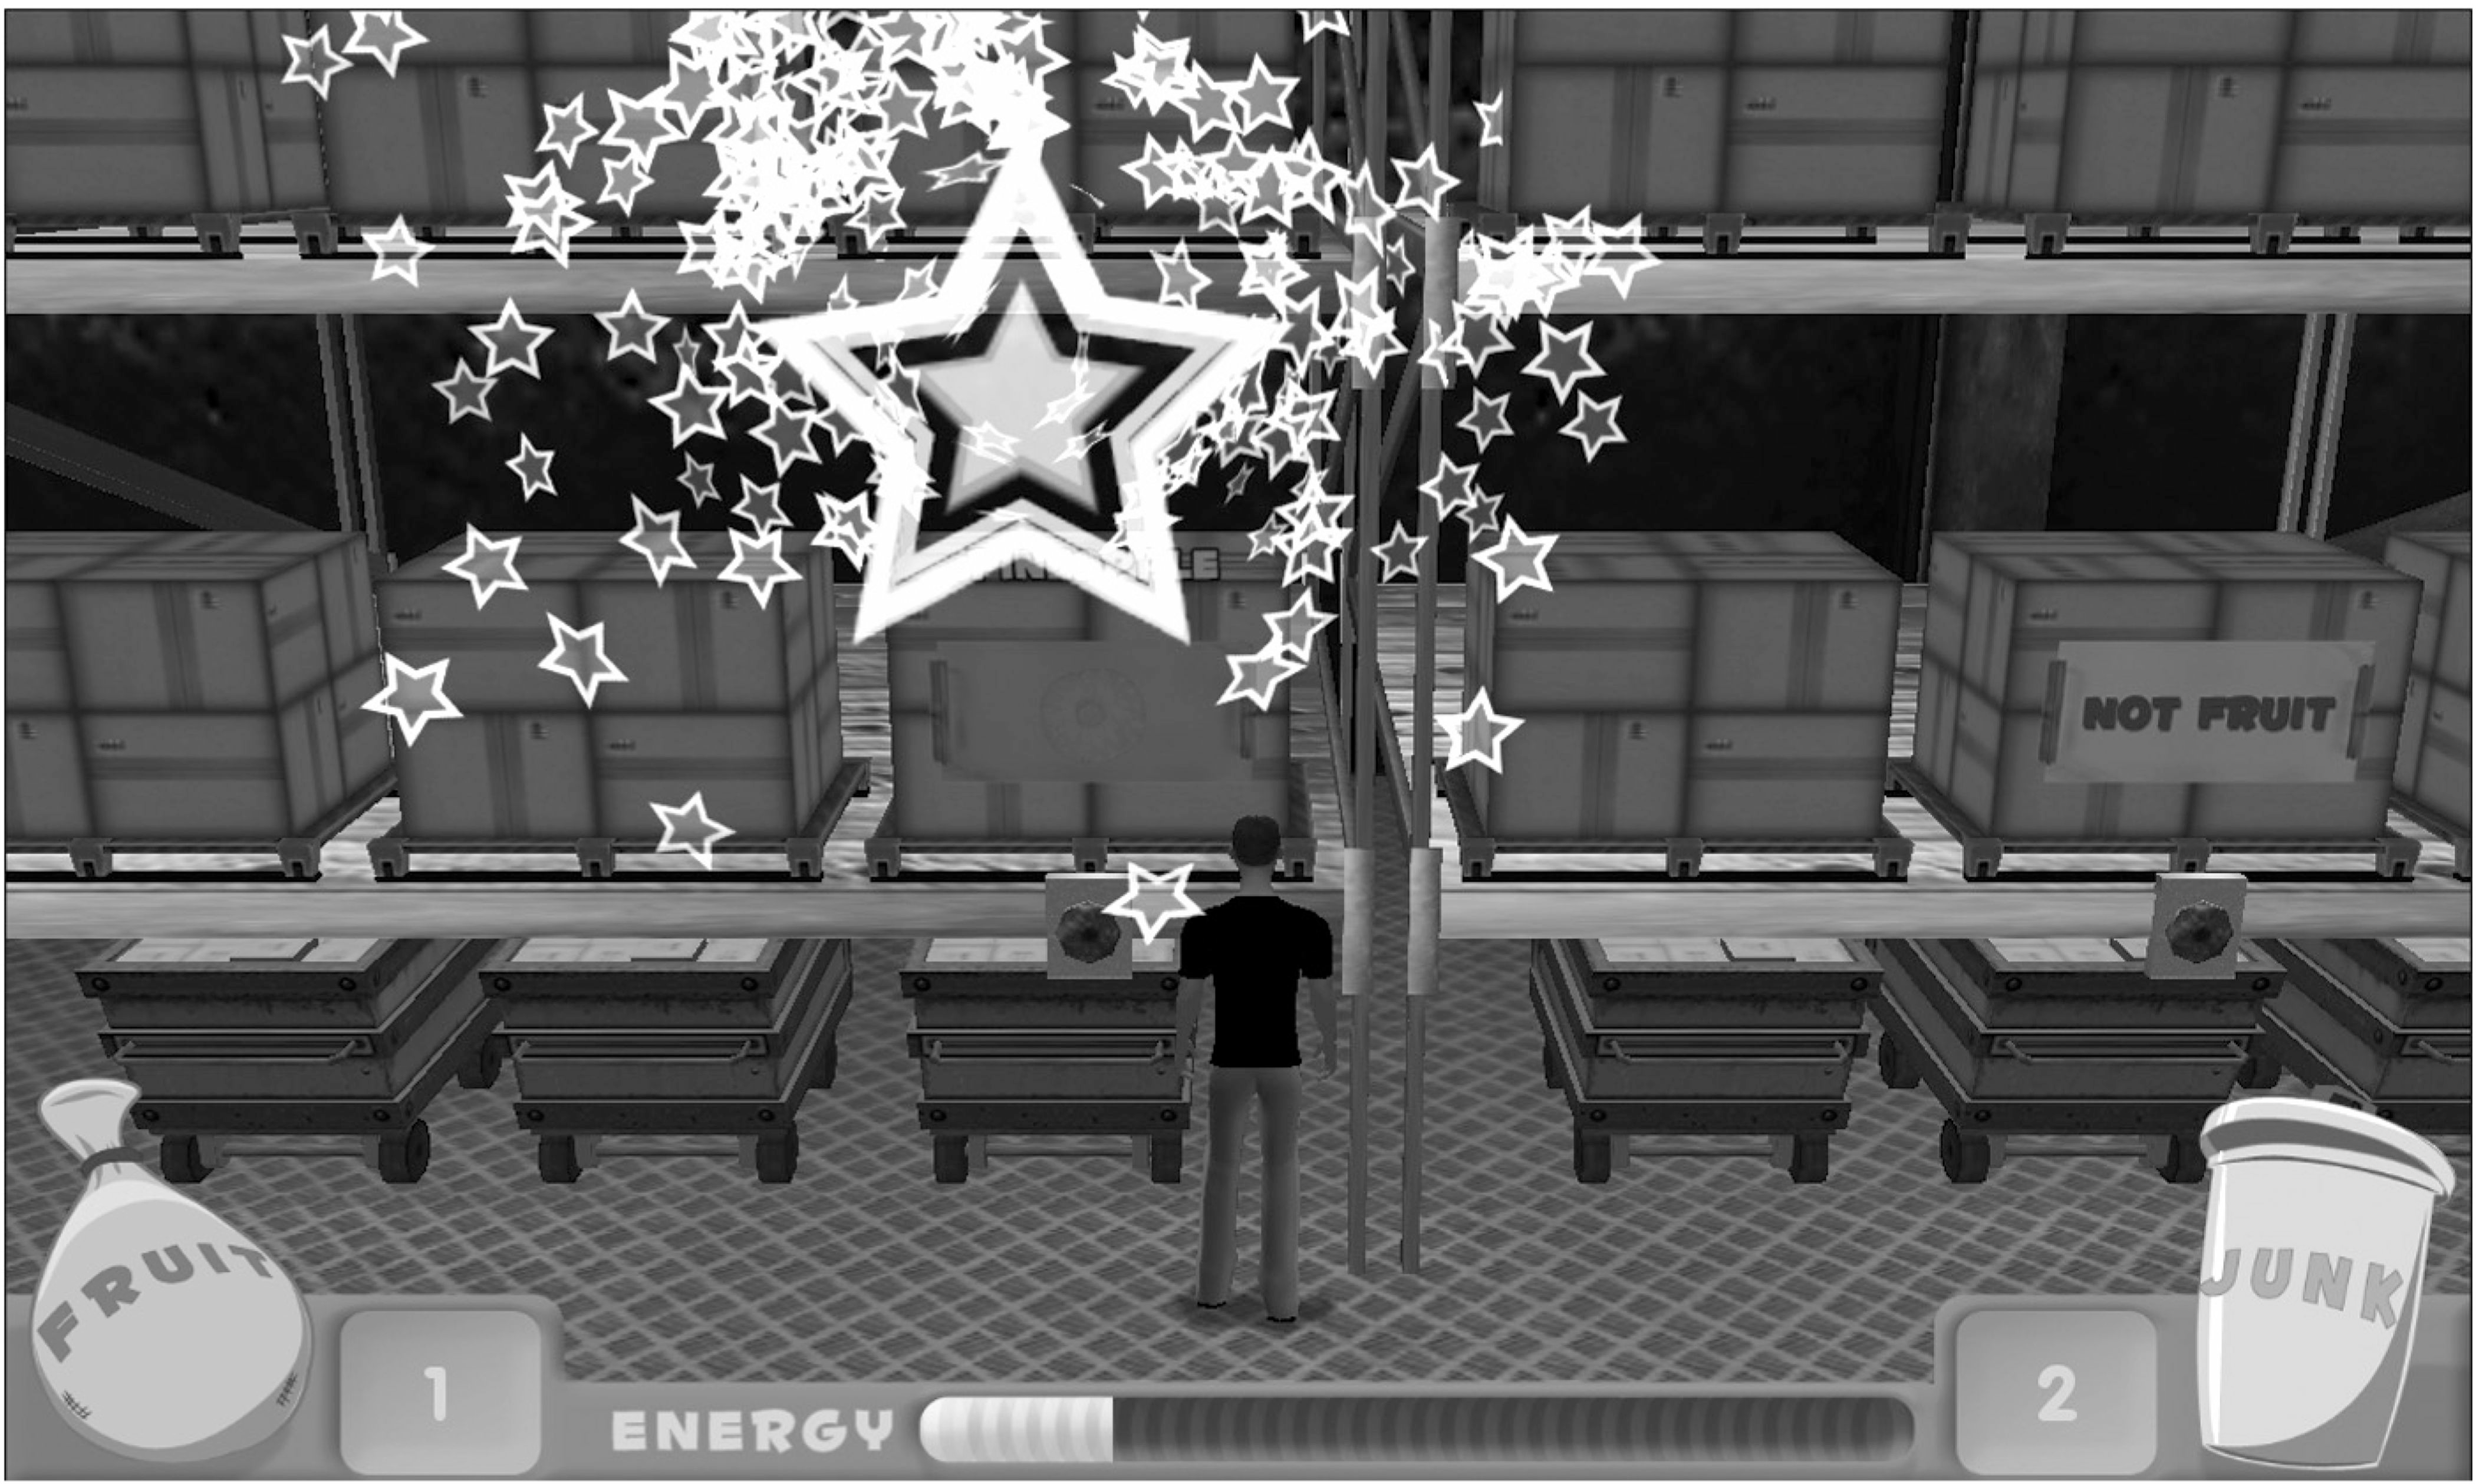
\includegraphics[scale=0.12]{./images/feedbacks}}
   	\caption{\label{Figure Feedback} Immediate Feedback by graphical effects \cite{Thompson10}}
\end{figure}
%-----------------------------------------------------------------%
\section{Interact with a Virtual Human}
The benefit of using virtual avatars for role playing training, comes from taking advantage of the fact that computer generated avatars can consistently present emotional stimuli at the will of the clinician \cite{Kim11}. Whereas the effectiveness of conventional role playing methods are often limited by the expressive capacity of the clinician/trainer. \\

Emotional processing, which is the ability to identify and recognize emotions through facial expressions, gestures, and tone of voice, is usually altered in schizophrenia and can have specific detrimental effects on functioning in everyday life \cite{Peyroux14}. For this reason the characters of the game need to show emotions to train the patient to recognise them. Futhermore, the avatar must have the ability to change emotion based on the actons of the patient.
 \subsection{Giving emotions to Virtual Humans}
The various facial behaviours and motions can be parameterized based on muscle actions. This set of parameters can then be used to represent the various facial expressions. To date, there have been two important and successful attempts in the creation of these parameter sets \cite{Bettadapura12}:
\begin{itemize}
\item The Facial Action Coding System (FACS) developed by Ekman and Friesen in 1977 \cite{Ekman77} and
\item The Facial Animation parameters (FAPs) which are a part of the MPEG-4 Synthetic/Natural Hybrid Coding (SNHC) standard, 1998 \cite{Pandzic03}.
\end{itemize}
\subsubsection{The Facial Action Coding System (FACS)}
Facial Action Coding involves identifying the various facial muscles that individually or in groups cause changes in facial behaviours. These changes in the face or underlying (one or more) muscles are called Action Units (AU). \\

AUs can be additive or non-additive. AUs are said to be additive if the appearance of each AU is independent. Contrastly, AUs are said to be non-additive if they modify each other’s appearance. Having defined these, representation of facial expressions becomes an easy task. Each expression can be represented as a combination of one or more additive or non-additive AUs. For example ‘fear’ can be represented as a combination of AUs 1, 2 and 26. Figure \ref{Figure FACs} show some examples of upper face AUs and the facial movements that they produce when presented in combination.
\subsubsection{The Facial Animation Parameters (FAPs)}
The Moving Pictures Experts Group (MPEG) introduced the Facial Animation (FA) specifications in the MPEG-4 standard. Version 1 of the MPEG-4 standard became the international standard in 1999. It supports facial animation by providing Facial Animation Parameters (FAPs).\\

The MPEG-4 defines a face model in its neutral state to have a specific set of properties like a) all face muscles are relaxed; b) eyelids are tangent to the iris; c) pupil is 1/3rd the diameter of the iris and so on. Key features like eye separation, iris diameter, etc are defined on this neutral face model.\\

The standard also defines 84 key feature points (FPs) on the neutral face and the movement of the FPs is used to animate the faces. Figure \ref{Figure FAPs} shows the location of the 84 FPs on a neutral face as defined by the MPEG-4 standard.\\

68 FAPs are defined by the MPEG-4. They are a set of parameters that represent a complete set of facial actions along with head-motion, tongue, eye and mouth control. The FAP value indicates the magnitude of the FAP which in turn indicates the magnitude of the deformation that is caused on the neutral model.

\begin{figure}[!h]
   	\centerline{\includegraphics[scale=0.4]{./images/facs}}
   	\caption{\label{Figure FACs} Some of the upper face AUs and their combinations \cite{Tian01}}
\end{figure}
\begin{figure}[!h]
   	\centerline{\includegraphics[scale=0.45]{./images/mpeg4}}
   	\caption{\label{Figure FAPs} The 84 Feature Points (FPs) defined on a neutral face \cite{Pandzic03}}
\end{figure}
\subsection{Patient's interactions}
There are different methods in which the patient can interact with the characters of the game. The simplest is to suggest several actions from which he must choose. This is what has been done in the RC2S program \cite{Peyroux14}. During the simulation scene, the patient has to choose a pattern of behavior(among those proposed) (see Figure \ref{Figure RC2S}). The social interaction scene follows a predefined but flexible decision tree where the patient’s choice influences upcoming interactions. For each interaction, three types of behaviors are suggested based on models from several social-skill training or self-affirmation programs: passive, aggressive or assertive behavior.\\

\begin{figure}[h]
   	%\centerline{\includegraphics[width=\textwidth]{./images/RC2S_long}}
   	\centerline{\includegraphics[scale=0.75]{./images/RC2S}}
   	\caption{\label{Figure RC2S} Images from the RC2S program \cite{Peyroux14}}
\end{figure}

This solution is simple to perform but it does not take into account the emotional state of the patient. From a therapeutic point of view, it would be interesting to adapt the scenario to the emotions of the patient in real time. This is the solution which has been explored in the game PlayMancer \cite{Fernandez12}, a serious video game designed to remediate attitudinal, behavioural and emotional processes of patients with impulse-related disorders. \\ 

Several new components were integrated in this video game platform, such as biosensors (galvanic skin response, oxygen saturation, heart rate (HR) and HR variation, skin temperature, breathing frequency), measured by a stationary measurement system based on the MobiHealth Mobile\textsuperscript{TM} system, and emotion recognition (anger, joy, boredom) feature extraction algorithms. Physiological reactivity and emotional recognition continuously track the emotional state of the player along the video game, while the game automatically responds in return by modifying aspects of the game play difficulty. \\

A pilot test was conducted to analyse the usability and comfort when using the video game along with the multiple connected biosensors.This found a mean of the average score estimation of 84.1\% (SD 13.2) in the average usability scores (as measured by Brooke's System Usability Scale: SUS). \\

Although the latter solution attained good results, there is a more discreet solution using emotion recognition via face and/or voice recognition systems. A study \cite{Busso04} has shown that the system based on facial expression gave better performance than that based on just acoustic information for the emotions considered. Results also show that when these two modalities are fused, the performance and the robustness of the emotion recognition system improved measurably.
\\

In the SimSensei Kiosk \cite{DeVault14} (a multimodal research platform for realtime assessment of distress indicators), the MultiSense framework was used as a perception system (see Figure \ref{Figure visio}). The system automatically tracks and analyzes in real-time facial expressions, body posture, acoustic features, linguistic patterns and higher-level behavior descriptors (e.g. attention and fidgeting). These informative signals are broadcasted to another component of SimSensei Kiosk to inform the virtual human of the state and actions of the participant and assist with turn taking, listening feedback, and building rapport by providing appropriate non-verbal feedback. \\
\begin{figure}[h]
   	\centerline{\includegraphics[scale=0.28]{./images/simsensei}}
   	\caption{\label{Figure visio} Multisense system \cite{DeVault14}}
\end{figure}
%-----------------------------------------------------------------%
\section{Variation of the scenarios}
The standard approach to incorporating storytelling into a computer system is to script a story at design time and then have the story's script execute without variation at run-time. If a computer system uses a scripted story, its ability to adapt to the user's interactions is limited. \cite{Riedl10}\\

In educational and training applications, a limited number of stories or permutations of a single story, limits the ability of the system to adapt to a learner's needs. Interactive Storytelling is a branch of Artificial Intelligence that deals with narrative objects (literary, videogames, film) to understand, analyze or generate them by providing techniques that can be implemented by computer programs. For example, Narrative Generation techniques are designed to create multiple different scenarios from the same initial narrative data. Mostly based on planning techniques \cite{Young99}, the recent narrative generation systems can also fall under the logic programming area \cite{Bosser10}.
\subsection{Planning techniques}
The generation of narratives can be seen as a knowledge-based planning problem with associated issues concerning representation and real-time performance. Planning was initially proposed for Interactive Storytelling in \cite{Young99}, and since then it has emerged as the dominant technology for Interactive Storytelling prototype systems. A number of factors have contributed to this: one is the apparent natural fit between narratives and plans which enables narratives to be naturally modelled as a sequence of actions; another is that plans embed key features including causality among story events.\\

Hierarchical Task Network (HTN) planning \cite{Erol94} has been adapted to dynamically generate the character roles, by interleaving planning and execution, which supports dynamic interaction between actors, as well as user intervention in the unfolding plot \cite{Cavazza02}. This way, characters’ roles, rather than a centralised plot model, serve as the main driver for narrative generation. From a technical perspective these roles display an internal structure, which is also task-based, with an implicit level of intentions predicated on the story structure.\\

Throughout the narrative genres that have served to illustrate research in interactive narrative, there has been a prevalence of those genres based on actions and situations rather than the psychological relations between agents. One notable exception has been : Fa\c cade \cite{Mateas05}, a first-person, real-time, one-act interactive drama. It involved three major research efforts: designing ways to deconstruct a dramatic narrative into a hierarchy of story and behaviour pieces; engineering an AI system that responds to and integrates the player’s moment-by-moment interactions to reconstruct a real-time dramatic performance from those pieces; and understanding how to write an engaging, compelling story within this new organizational framework.\\
In his thesis, Pizzi \cite{Pizzi11} described a prototype in which characters’ behaviour is driven by a real-time heuristic search planner that applies operators whose content is based on a specific inventory of feelings.\\

After many years of using planning for narrative generation, research then concentrated on solving some remaining problems. Porteous et al. \cite{Porteous10} for example, suggested a solution to best control the shape of the narration generated and give a better support for real-time interactive performance. Their approach was to specify narrative control knowledge for a given story world using state trajectory constraints. Then to treat these state constraints as landmarks, using them to decompose narrative generation, in order to address scalability issues and the goal of real-time performance in larger story domains.\\

Riedl and Young \cite{Riedl10} suggested a solution to generate a sound and believable sequence of character actions that transforms an initial world state into a world state in which goal propositions hold. Their refinement search planning algorithm: Intent-based Partial Order Causal Link (IPOCL) planner, in addition to creating believable plot progression, reasons about character intentionality. It indentifies possible character goals that explain their actions and creates plan structures that explain why those characters commit to their goals.\\

Even if planning has emerged as the dominant technology, featuring in a number of prototype systems, more recently, Linear Logic has been proposed as a suitable representational model for narratives because it supports causality \cite{Bosser10}. Masseron et al. \cite{Masseron93} have established how Linear Logic formalisation could support planning and how the properties of Linear Logic made it so that a proof in Linear Logic could be equated to a plan.
\subsection{Linear logic programming}
In their paper, Martens et al. \cite{Martens13} explore the use of Linear Logic programming for story generation. They use the language Celf \cite{Schack08} to represent narrative knowledge, and its own querying mechanism to generate story instances, through a number of proof terms.\\

Celf programs are normally divided into two main parts: a \textbf{signature}, which is a declaration of type and terms constants describing data and transitions, and \textbf{query directives}, defining the problem for which Celf will try to find solutions.\\

Figure \ref{Figure celf} shows an example of Celf program representative of the form used to model narrative, and composed of signature and a query of 100 attempts to generate stories ending with the death of the character Emma (line 22). \\

The story elements available as well as the states of the story are the \textbf{narrative resources} (lines 1-5). Transforming events occuring in the narrative (such as resource creation and consumption) are called \textbf{narrative actions} (lines 6-14). The initial narratice environment is describes with the type init (line 15).\\

Once the narrative is modelled, it is run using Celf and the proof-terms obtained are post-processed for causality analysis. They also developed CelfToGraph, that automatically transforms proof terms generated by Celf into directed acyclic graphs. Such graphs represent narrative plots, structured by narrative causality, where nodes are narrative actions and edges represent inferred causality relationships.\\

The code described allows to generate 72 different narrative sequences for 100 attempts. After an automatic comparison of the corresponding plots using CelfToGraph, they can exhibit 41 different plots, meaning that a number of different narrative sequences share the same causal structures. This allows the characterisation of classes of true story variants.
\begin{figure}[!h]
   	\centerline{\includegraphics[scale=0.6]{./images/celf}}
   	\caption{\label{Figure celf} Example of the Celf program used \cite{Martens13}}
\end{figure}
%-----------------------------------------------------------------%
\section{Conclusion}
Most people with schizophrenia suffer from a strong social isolation due to the fact that they have difficulty communicating, even in the most mundane situations of daily life. Social skills training teaches the patients how to extend their behavioral repertoires in order to be able to communicate and regain some independance.\\

Serious games can be a great asset for social skills training as they provide a safe environment in which the patients can practice social interaction without the repercussions of emotional frustration and feeling of failure expected in the real world. The entertainment also increases their motivation and hold the patient's attention, which can increase the effectiveness of the treatment. \\

The recognition of facial expressions is usually altered in schizophrenia, for this reason the characters of the game need to show emotions in order to train the patient to recognise them. During the internship I will use the HapFACS \cite{Amini13}, a open source software and API developed by the University of Miami (see Figure \ref{Figure HapFACS}). It generats FACS-based facial expressions on 3D virtual characters that have accompanying lip synchronized animation abilities. With the accessible HapFACS API, it is possible to animate speaking virtual characters with real-time realistic facial expressions, and embed these expressive characters into other(s) application(s). \\

There are different methods in which the patient can interact with the characters of the game. The simplest is to suggest several actions from which he must choose (see Figure \ref{Figure RC2S}). It is also possible to use biosensors and use physiological reactivity and emotional recognition to track the emotional state of the player. Another more discreet solution is to use face and voice recognition. It is possible to use these solutions on their own or to combine them for better results. I am yet to make a decision on the technique that will be used during the internship. These different methods will have to be discussed with the psychiatric team in order to make a descision. \\

It is particularly interesting from a therapeutic point of view, to be able to vary the scenarios of the game to lead patients to respond to unforeseen situations in a safe environment. Patients also need to train regularly but if they always do the same exercices they will lose interest and their training will not be efficient. Narrative generation is a solution to generate scenarios. The program TeLLer \footnote{Project TeLLer. Page maintained by Jo\~{a}o F. Ferreira (University of Teesside) gathering programs to test the use of linear logic for computational narrative. https://github.com/jff/TeLLer.} is a collection of tools that explore the use of linear logic for narrative generation. The first tool allows the program to generate stories based on knowledge that is provided to the system. The second tool is used to generate a direct graph where nodes are narrative actions and edges represent inferred causality relationships. \\

As a concrete example, imagine a scene where the patient has to collect medication at the pharmacy. He or she will have to choose the correct behaviour in order to achieve his or her target. The speech provided by the pharmacist will be managed by Teller, his facial expression as well as the lip synchronization will be managed by HapFACS (see Figure \ref{Figure finalDiagram}).\\
\begin{figure}[h]
   	\centerline{\includegraphics[scale=0.4]{./images/hapfacsAPI}}
   	\caption{\label{Figure HapFACS} HapFACS interface \cite{Amini13}}
\end{figure}
\begin{figure}[h]
   	\centerline{\includegraphics[scale=0.4]{./images/final_diagram}}
   	\caption{\label{Figure finalDiagram} Diagram}
\end{figure}


%*****************************************************************%
\newpage
\bibliographystyle{abbrv}
\bibliography{ref}
\end{document}
